\documentclass [10pt,a4paper]{article}
\usepackage[danish]{babel}
\usepackage{a4wide}
\usepackage[T1]{fontenc}
\usepackage[utf8x]{inputenc}
\usepackage{amsmath}
\usepackage{amsfonts}
\usepackage{fancyhdr}
\usepackage{ucs}
\usepackage{graphicx}
\usepackage{listings}
\usepackage{color}

\pagestyle{fancy}
\fancyhead[LO]{Michael Thulin, Philip Munksgaard}
\fancyhead[RO]{Maskinarkitektur: G-Opgave 2}
\fancyfoot[CO]{\thepage}


\title{G-Opgave 2}
\author{Michael Thulin, Philip Munksgaard}

\begin{document}
\maketitle

\section{Pipeline-arkitektur}

\subsection{Implementering af pipelining}

Vi tog udgangspunkt i figur 4.60 i COD, og implementerede pipelining i
vores kredsløb fra G1. Først opdelte vi vores gamle kredsløb i stages og lavede de
forskellige registre til at indeholde data i de forskellige
stages. 

\subsection{Ny control}

For at understøtte vores nye stages, samt simplificere kredsløbet og
stage-registrene, har vi valgt at konsolidere control-linjerne og
samle dem i forhold til de stages hvori de skal
bruges. Control-enheden har fire output, sign-extend, jump, link og
control-linjen. \newline
Control-linjen består af alle controllinjerne, som så senere bliver
delt op og puttet ind i de rigtige trin i pipelinen.

Jump og link-linjerne bruges i j, jal og jr. og er beskrevet nedenfor.

\begin{table}
  \centering
  \begin{tabular}{ c | c | c }
    \textbf{Bit} & \textbf{Operation} & \textbf{Gruppe} \\
    0 & AluOP & EX \\
    1 & Branch & M \\
    2 & MemWrite & M \\
    3 & MemRead & M \\
    4 & RegWrite & WB \\
    5 & MemToReg & WB \\
    6 & ALUSrc & EX \\
    7 & RegDst & EX \\
    8 & AluImmediate0 & EX \\
    9 & AluImmediate1 & EX \\
    10 & AluImmediate2 & EX \\
    11 & AluImmediate3 & EX \\
  \end{tabular}
  \caption{Oversigt over bits på control-linjen fra control-enheden}
\end{table}

\begin{table}
  \centering
  \begin{tabular}{ c | c }
    \textbf{Bit} & \textbf{Betydning} \\
    0 & ALUOp \\
    1 & Branch \\
    2 & ALUsrc \\
    3 & RegDst \\
    4 & ALUImmediate0 \\
    5 & ALUImmediate1 \\
    6 & ALUImmediate2 \\
    7 & ALUImmediate3 \\
  \end{tabular}
  \caption{Oversigt over control-bits på EX-trinnet i pipelinen}
\end{table}

\begin{table}
  \centering
  \begin{tabular}{ c | c }
    \textbf{Bit} & \textbf{Betydning} \\
    0 & MemWrite \\
    1 & MemRead \\
  \end{tabular}
  \caption{Oversigt over control-bits på M-trinnet i pipelinen}
\end{table}

\begin{table}
  \centering
  \begin{tabular}{ c | c }
    \textbf{Bit} & \textbf{Betydning} \\
    0 & RegWrite \\
    1 & MemToReg \\
  \end{tabular}
  \caption{Oversigt over control-bits på WB-trinnet i pipelinen}
\end{table}

\subsection{Forwarding}

I vores implementation af forwarding enheden har vi bare fulgt bogens
beskrivelser fra side 366 til side 371. 

\subsection{Hazard detection og stalls}

Vi fulgte beskrivelsen af hazard detection på side 372 i vores
hazard detector. Når vi detekterer en hazard, får vi en høj på stall
linjen. Når stall-linjen er høj, indsætter vi nop i ID/EX trinnet (ved
hjælp af en multiplexor) og vi staller IF/ID registret og program
counteren.

\subsection{Implementering af j, jal og jr}

Vores implementation af j-instruktionen følger bogens eksempel og
bruger jump-control linjen fra control-enheden. Når denne linje er
høj, springer program counteren og vi staller IF/ID registret.

Jal virker ved at vi springer i ID trinnet og indsætter at vi skal
skrive program counter + 4 i register 31 i vores pipeline.

Jr springer i EX-trinnet, og virker ved at vi læser register 31 og
springer på samme måde. Vi har ændret i ALUcontrol enheden så vi kan
smide en høj værdi på jr-linjen, som springer til den adresse vi har
fået ud fra registret.

\section{Implementation af primes.c i assembler}

Koden kan ses i bilag B.

\begin{table}
  \caption{Oversigt over hvilke registrer der bruges til hvad i
    primes.asm}
  \centering
  \begin{tabular}{ c | c }
    \textbf{Bit} & \textbf{Betydning} \\
    \$s0 & i \\
    \$s1 & p \\
    \$s2 & idx \\
    \$s3 & n \\
    \$s4 & primes \\
  \end{tabular}
\end{table}

\clearpage

\section*{Bilag A: Figurer af udvalgte delkredsløb}

\begin{figure}[h!]
  \centering  
    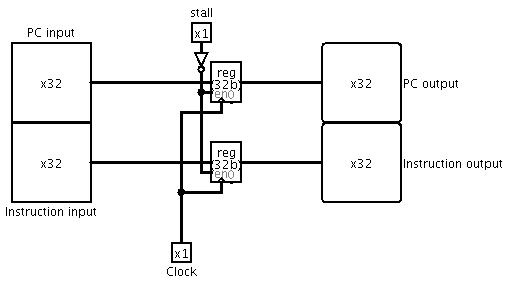
\includegraphics[scale=0.7]{ifid.png}
  \caption{IF/ID registrerne.}
\end{figure}

\begin{figure}[h!]
  \centering  
    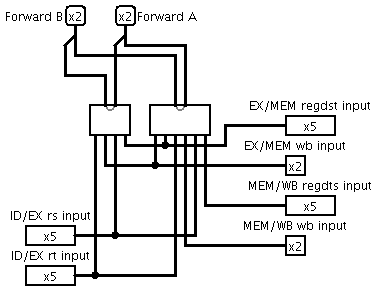
\includegraphics[scale=0.7]{forwarding.png}
  \caption{Vores forwarding enhed.}
\end{figure}

\begin{figure}[h!]
  \centering  
    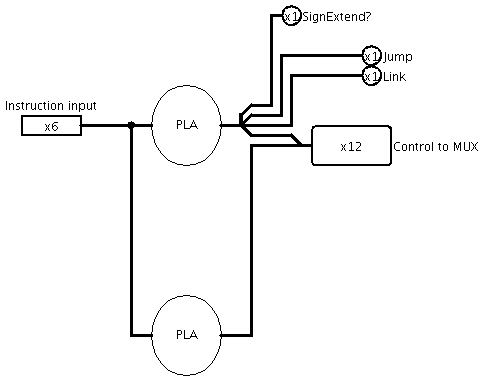
\includegraphics[scale=0.7]{control.png}
  \caption{Vores control komponent.}
\end{figure}

\begin{figure}[h!]
  \centering  
    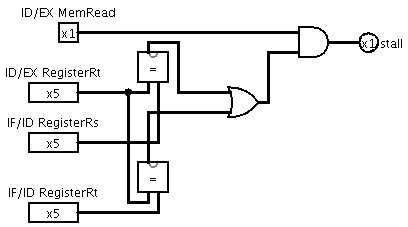
\includegraphics[scale=0.7]{hazard.png}
  \caption{Vores hazard detection enhed.}
\end{figure}


\clearpage

\section*{Bilag B: Primes.c i assembler}
\lstinputlisting[language=Assembler]{primes.asm}


\end{document}
